
\documentclass[9pt]{pnas-new}
% Use the lineno option to display guide line numbers if required.
% Note that the use of elements such as single-column equations
% may affect the guide line number alignment. 

%\RequirePackage[english,slovene]{babel} % when writing in slovene
\RequirePackage[slovene,english]{babel} % when writing in english
\DeclareUnicodeCharacter{202F}{ }
\templatetype{pnasresearcharticle} % Choose template 
% {pnasresearcharticle} = Template for a two-column research article
% {pnasmathematics} = Template for a one-column mathematics article
% {pnasinvited} = Template for a PNAS invited submission

\selectlanguage{english}
%\etal{in sod.} % comment out when writing in english
%\renewcommand{\Authands}{ in } % comment out when writing in english
%\renewcommand{\Authand}{ in } % comment out when writing in english

\newcommand{\set}[1]{\ensuremath{\mathbf{#1}}}
\renewcommand{\vec}[1]{\ensuremath{\mathbf{#1}}}
\newcommand{\uvec}[1]{\ensuremath{\hat{\vec{#1}}}}
\newcommand{\const}[1]{{\ensuremath{\kappa_\mathrm{#1}}}} 
\usepackage{caption}
\usepackage{subcaption}
\usepackage{gensymb}
\newcommand{\num}[1]{#1}

\graphicspath{{./fig/}}

\title{Simulation of group behaviour during a protest}

% Use letters for affiliations, numbers to show equal authorship (if applicable) and to indicate the corresponding author
\author{Nik Čadež}
\author{Pedro Nuno Ferreira Moura de Macedo}
\author{Primož Mihelak}
\author{Luka Bajić}

\affil{Collective behaviour course research seminar report} 

% Please give the surname of the lead author for the running footer
\leadauthor{Čadež} 

\selectlanguage{english}

% Please add here a significance statement to explain the relevance of your work
\significancestatement{By conducting simulations of protests using various models for different subgroups of people, we hope to gain some insight into group behaviour during such events, that might make them logistically easier to organize/control in the future.}{Simulation | group behaviour | group dynamics}

\selectlanguage{english}

% Please include corresponding author, author contribution and author declaration information
%\authorcontributions{Please provide details of author contributions here.}
%\authordeclaration{Please declare any conflict of interest here.}
%\equalauthors{\textsuperscript{1}A.O.(Author One) and A.T. (Author Two) contributed equally to this work (remove if not applicable).}
%\correspondingauthor{\textsuperscript{2}To whom correspondence should be addressed. E-mail: author.two\@email.com}

% Keywords are not mandatory, but authors are strongly encouraged to provide them. If provided, please include two to five keywords, separated by the pipe symbol, e.g:
\keywords{Simulation | group behaviour | group dynamics} 

\begin{abstract}
The purpose of our project is to model the behaviour of a crowd during a protest as accurately as possible and attempt to observe the emerging behavioural patterns. At the start of a simulation we populate the scene with agents that belong in different subgroups (leader, protester, bystander), but eventually they can fluidly change between the groups based on various parameters, such as proneness to defection and recruitment. These parameters depend upon the distribution (in the sense of groups) of agents in an individual's field of view. The movement of the leader can either be manually controlled by the user, or determined by arbitrary goals within the topological map, while the other agents follow the leader when it appears in their field of vision, depending also on their aggression parameters. To give the simulation a practical use, we additionally allow the user to manually place police agents into the scene and observe how they impact the behaviour of the crowd. 
\end{abstract}

\dates{\textbf{\today}}
\program{BMA-RI}
\vol{2024/25}
\no{Group A} % group ID
%\fraca{FRIteza/201516.130}

\begin{document}

% Optional adjustment to line up main text (after abstract) of first page with line numbers, when using both lineno and twocolumn options.
% You should only change this length when you've finalised the article contents.
\verticaladjustment{-2pt}

\maketitle
\thispagestyle{firststyle}
\ifthenelse{\boolean{shortarticle}}{\ifthenelse{\boolean{singlecolumn}}{\abscontentformatted}{\abscontent}}{}

% If your first paragraph (i.e. with the \dropcap) contains a list environment (quote, quotation, theorem, definition, enumerate, itemize...), the line after the list may have some extra indentation. If this is the case, add \parshape=0 to the end of the list environment.
\dropcap{P}rotests are a widespread phenomenon involving typically large groups of people, oftentimes with different, or even conflicting goals between their respective subgroups. As such they are a fascinating subject for studies in various fields, from human psychology to group behaviour simulations, which was be our primary focus during the course of this project. 

\bigskip
The central idea for the project was inspired specifically by the 2020 protests in Ljubljana, that had a distinguishing feature of a prominent individual leader emerging and influencing the movement of the crowd, but we have attempted to make our model applicable more generally (for instance, with minor parameter adjustments, we should be able to easily model sports riots or other similar events with various subgroups).  

\section*{Related work}

Although there are many existing attempts to model protest behaviour, in terms of general structure, our project will primarily build on concepts proposed by Lemos, et. al. \cite{protests}. The basic idea is to split the agents into subgroups depending on their level of involvement with the protest. The proposed subgroups are:
\begin{itemize}
    \item active protesters, further divided by their level of aggression, 
    \item passive protesters - hereafter we refer to them as bystanders,
    \item police/crowd control agents: their primary goal is dispersing a crowd or redirecting it in a specific direction.
\end{itemize}

\bigskip
Clements and Fadai \cite{sportsriots} have developed a model that attempts to simulate emotional contagion in the context of a sports riot. Although our problem is slightly different in nature, we do use the same principles of defection and recruitment in order to create approximately realistic transitions from active protesters to bystanders and vice versa, depending on what group the majority of agents in the current field of view of an individual belong to. 

\bigskip
To make simulations appear as realistic as possible, it is necessary to give all agents movement parameters that aim to mimic human behaviour in crowded environments. The forces that impact each agent are described, for instance by Itatani and Pelechano \cite{socialcrowdsimulation} and are divided into: collision avoidance force, wall repulsion force, end-position seeking force, group dynamics force and anticipatory collision avoidance force. 

\section*{Methods}

Implementation of the model was done in Unity, in a 2-dimensional space observed from bird's-eye perspective. While creating the topological map of Ljubljana into which the agents will later be placed, we had to ensure the correct scale and proportions. We used Google Maps for this step and we took into account the estimated maximum numbers of people that can fit into spaces of particular dimensions. In other words, we attempted to create an environment that's as realistic as possible, so that the obtained results will potentially be useful in various practical applications. 

\subsection*{Subgroups}
In addition to Lemos' subgroups \cite{protests}, we also implemented the concept of a leader and for this purpose we divided the simulation into two modes:
\begin{itemize}
    \item user manually controls the movement of a single leader: this can be used for instance to recreate very specific movement from real-life situations.
    \item multiple local leaders emerge spontaneously within the group and form a hierarchy of leaders.
\end{itemize}

\subsection*{Vision}
To give our agents awareness of their surroundings, we also need to model vision (example of a visualization is shown in figure \ref{vision}). This consists of two parts: 
\begin{itemize}
    \item field of view to model a human's eyesight. Default value is \begin{math}60\degree\end{math}, with a distance of 24 Unity units.
    \item peripersonal space to model a human's ability to feel a presence outside of their field of view, if the distance is small enough. Default value is \begin{math}300\degree\end{math}, with a distance of 1.6 Unity units.
\end{itemize}

\begin{figure}[H]
\centering
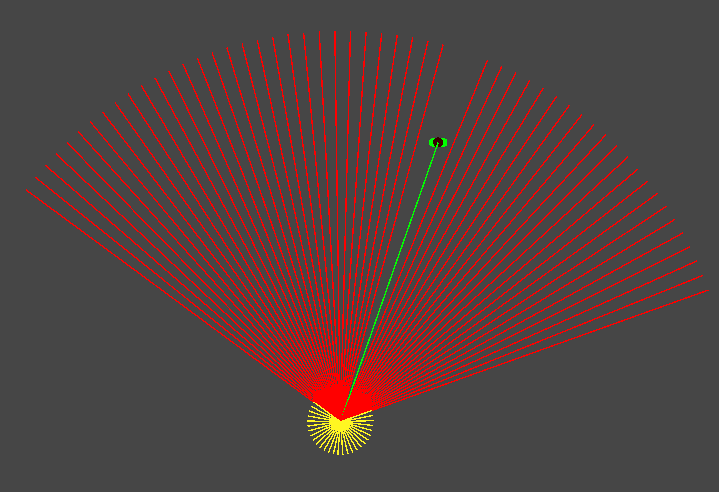
\includegraphics[width=0.95\columnwidth]{vision.png}
\caption{Visualization of the implemented vision: red rays represent field of vision, yellow rays represent peripersonal space, green ray represents a detected agent.}
\label{vision}
\end{figure}

\subsection*{Movement}

Agents switch between two main states during the course of the simulation: standing still and in-motion. For this purpose we have come up with a restlessness parameter that gradually increases in agents that are standing still and once it reaches a certain threshold, the agent begins to move. To ensure that not all agents start and stop moving at the same time, it is paramount that the restlessness parameter is increased randomly (which based on our observations of various protest footage is the case for humans as well). 

\bigskip
We deviate from Itatani \cite{socialcrowdsimulation} when it comes to End-Position-Seeking-Force, because the nature of our problem is considerably different. Our agents do not have an end position per se, therefore we have to set this value either to the position of the leader (in case a particular agent is currently following the leader), or an arbitrary nearby point in space (if an agent is not attached to the leader). The point in space is calulated differently for bystenders and protesters, since their movements typically have inherently different purposes: bystanders tend to move away from the heated crowd, while the active protesters usually attempt to join in. 


\section*{Results}

So far we have implemented a simulation that incorporates four groups of agents in the same scene and we have defined different movement and interaction parameters for each of them. The agents are shown in figure, placed in an environment that is essentially a Unity representation of topological map of a portion of Ljubljana (shown in figure \ref{fig2}). We have decided to focus on an area with two main squares and a few narrow streets in-between and around them, in order to observe crowd behavior in different sized environments. We have also calculated an approximate amount of agents that could realistically fit into a square of this size. 

\begin{figure}[H]
\centering
\begin{subfigure}{.5\textwidth}
  \centering
  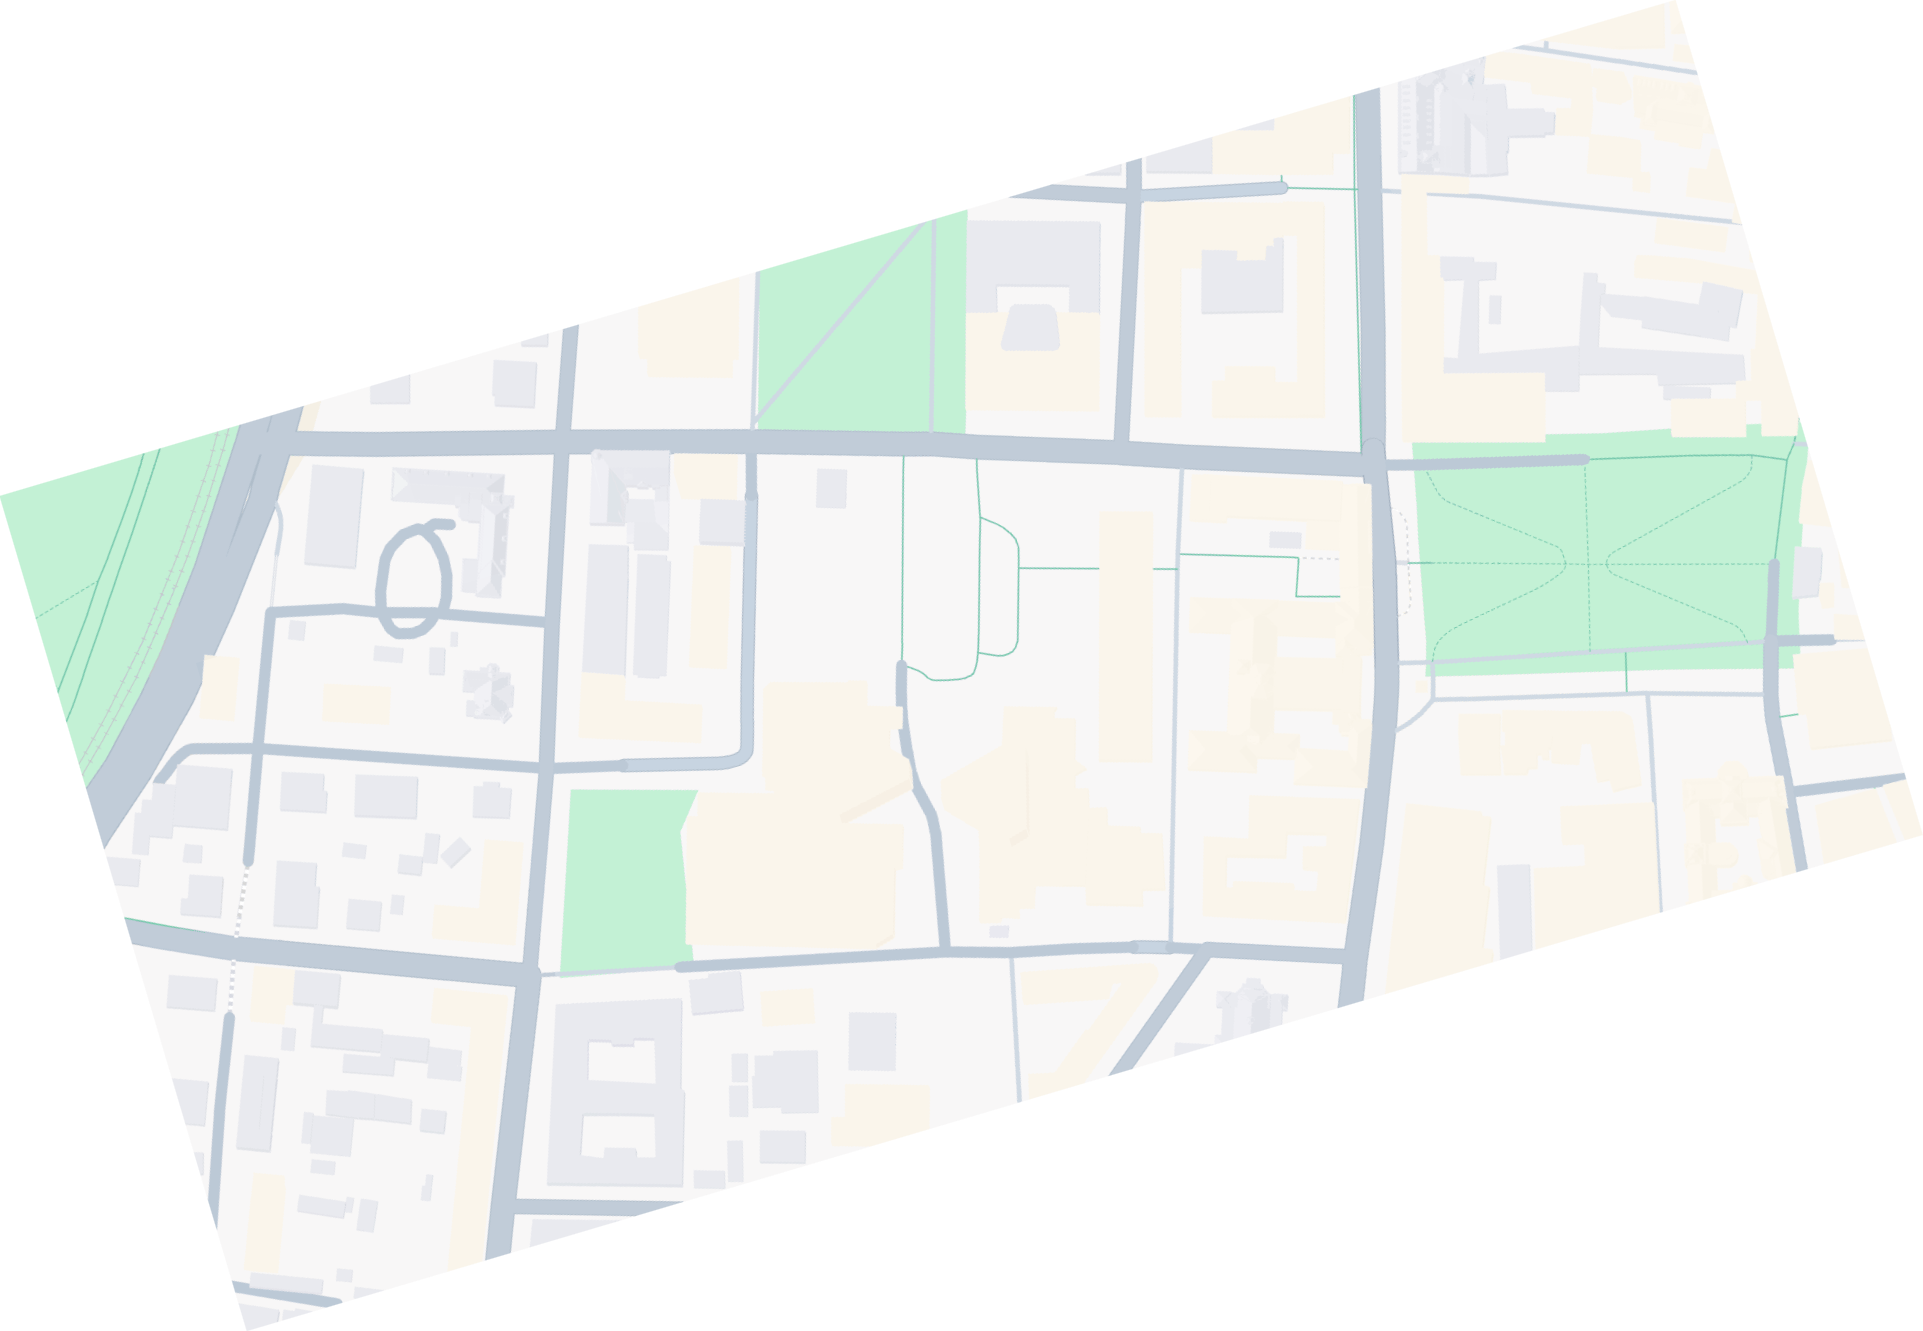
\includegraphics[width=0.95\columnwidth]{finalmap_rotated.png}
  \caption{Google map image without labels}
  \label{fig:sub1}
\end{subfigure}%
\begin{subfigure}{.5\textwidth}
  \centering
  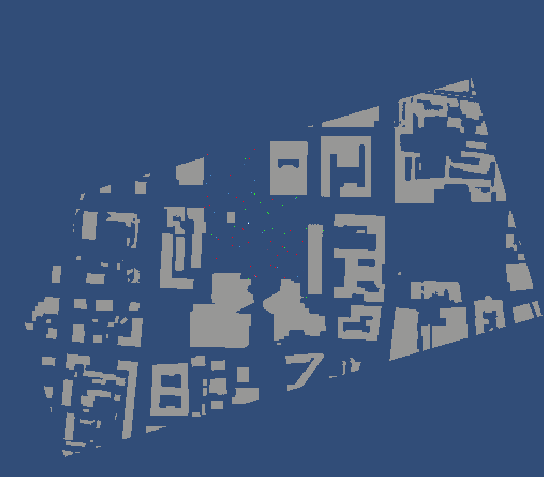
\includegraphics[width=0.95\columnwidth]{fullmap.png}
  \caption{Generated map in Unity}
  \label{fig:sub2}
\end{subfigure}
\caption{Example of a transformation of a Google map image into a Unity map. The rotation was added to make the simulation more easy to observe. }
\label{fig2}
\end{figure}

The simulation is designed to start with a fixed number of agents (default value is 200), one being the leader, the rest being randomly distributed between protesters and bystanders, as well as randomly positioned on the map. Additionally, the user can manually place a certain amount of police agents into the scene (upper bound is set to 50 by default) in straight lines to simulate barricades. 

\bigskip
One of the principal observations is that the end-position-seeking-behaviour correctly and realistically forms a group of protesters in the center of the crowd, while the bystanders seek to move away from the formed group. Emotional contagion ensures that if an individual bystander is surrounded by a group of protesters for a long enough period of time, it will eventually turn into a protester as well, with a relatively high likelihood. 

\bigskip
A hierarchy of leaders emerges spontaneously. Active protesters identify themselves as leaders with a very low probability and keep the role only a big enough number of surrounding agents begins to follow them. We use emotional contagion for deidentification in a similar manner as well. 


\section*{Discussion}

Most of the goals of the project were accomplished successfully, however we propose some potential improvements that are yet to be implemented: 
\begin{itemize}
\item current implementation of the map assumes buildings are the only structure that acts as a repulsive force on the agents. To increase realism, it would be necessary to also include other objects, such as trees, statues, etc.
\item solving the problem of displaying the agents' dimensions relative to building's dimensions (i.e. how to simultaneously show a big portion of the map while maintaining a clear vision of the agents).
\item developing an approach for police agents to find more optimal formations (e.g. by using genetic algorithms). 
\item introducing some uncertainty into vision might further improve the realism of the simulation - an agent should occasionally incorrectly recognize a protester as a bystander or vice versa, with a low, but non-zero probability. 
\end{itemize}


\acknow{NČ implemented agent movement, vision and interaction between different groups, PNM created the map and implemented the police agents, PM implemented transitions between groups (emotional contagion) and improved the visualization, LB did image processing for the map, implemented the baseline model and wrote the reports}
\showacknow % Display the acknowledgments section

% \pnasbreak splits and balances the columns before the references.
% If you see unexpected formatting errors, try commenting out this line
% as it can run into problems with floats and footnotes on the final page.
%\pnasbreak

\begin{multicols}{2}
\section*{\bibname}
 %Bibliography
\bibliography{./bib/bibliography}
\end{multicols}

\end{document}